\subsection{Jogos de Shannon}
\begin{frame}[allowframebreaks]
  \frametitle{Jogos de Shannon}
  \begin{itemize}
  \item Redundância está presente em todos lugares. Em um língua existe redundância no nível de sentenças, 
	no nível de palavras e no nível de caracteres.
  \item Exemplos:
	\begin{quote}
	``Não se ama duas vezes a mesma {\color{white}mulher}''. \\
	``A gratidão de quem recebe um benefício é bem menor que o prazer daquele de quem o {\color{white}faz}''. \\
	\hfill(Machado de Assis)
	\end{quote}
  \item Shannon percebeu isto e propôs uma maneira de estimar a entropia.
  \item Assuma o alfabeto `a' a `z' mais espaço (27 caracteres).
  \item Um caractere é dado a cata instante e uma pessoa deve adivinhar qual é o próximo.
                \begin{figure}[h!]
                \centering
                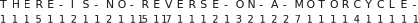
\includegraphics[width=0.75\textwidth]{images/shannonguessgame.pdf}
                \label{fig:shannonguessgame}
                \end{figure}
  \item O número de tentativas para adivinhar a letra correta pode ser vista como um `código' para a \textit{string}.
	Teremos assim um mapeamento de letras em inteiros:
	\begin{equation}
	C: \{'a','b','c', \ldots ,'z','\ '\} \rightarrow \{1,2,\ldots,27\}
	\end{equation}
  \item Usualmente o número de tentativas será pequeno. Aquilo que é mais dedutível terá maior probabilidade e menor número de tentativas
	serão necessárias.
  \item Seja $g_t$ o número de tentativas até acertar na posição $t$, então $\log g_t$ será o número de bits necessários para
	representar $g_t$.
  \item A taxa de entropia deste processo é
	\begin{equation}
	\hat{H}(X) \approx \frac{1}{n} \sum_{t=1}^{n} \log g_t .
	\end{equation}
  \item Supondo que $x_1,x_2,\ldots$ é um processo estocástico com taxa de entropia da forma $H(X_t \mid X_{t-1}, \ldots, X_1)$, então
	$p(x_t \mid x_{t-1}, x_{t-2}, \ldots, x_1)$ é a probabilidade da letra $x_t$ no instante $t$. Teremos então
	\begin{equation}
	g_t \approx \frac{1}{p(x_t \mid x_{t-1}, x_{t-2}, \ldots, x_1)} .
	\end{equation}
  \item Ao realizar tal codificação teremos que os números pequenos serão muito mais frequentes do que os grandes. Para o
	exemplo anterior, `There is no reverse on a motorcycle', será associada a seguinte sequência de símbolos:
	1, 1, 1, 5, 1, 1, 2, 1, 1, 2, 1, 1, 15, 1, 17, 1, 1, 1, 2, 1, 3, 2, 1, 2, 2, 7, 1, 1, 1, 1, 4, 1, 1, 1, 1, 1.
  \item Devemos ter um bom resultado na compressão desta sequência.
  \item Para realizar a decodificação precisaremos de um gêmeo idêntico, que faça as mesmas adivinhações, ou seja, realizará $g_t$ 
	tentativas até acertar.
  \item Outra alternativa seria criar uma longa tabela com todos históricos possíveis e memorizar o esquema as tentativas que um humano faria.
	Para uma \textit{string} de tamanho $L$ temos $27^L$ combinações, tornando esta abordagem impraticável.
  \item Uma alternativa viável seria considerar $P(X_t \mid X_{t-1}, \ldots, X_1) \approx P(X_t \mid T(X_1, \ldots, X_{t-1}))$, onde
	$T(X_1, \ldots, X_{t-1})$ é uma estatística sobre as $t-1$ amostras passadas e a cada instante basta ajustar a estatística.
  \item Este esquema introduzido por Shannon nos anos 1950 é a base para a codificação aritmética.
  \end{itemize}
\end{frame}


\subsection{Codificação Aritmética}
\begin{frame}[allowframebreaks]
  \frametitle{Codificação Aritmética}
  \begin{itemize}
  \item Utilizada em compressão de documentos: DjVU, PDF, JPEG.
  \item Assumir o seguinte modelo probabilístico da fonte:
	\begin{equation}
	p(x_{1:n}) = \prod_{i=1}^{n} p(x_i) \quad \text{i.i.d.}
	\end{equation}
	ou, de forma alternativa,
	\begin{equation}
	p(x_{1:n}) = p(x_1) \prod_{i=2}^{n} p(x_i \mid x_{i-1}) \quad \text{modelos de Markov de 1a ordem}.
	\end{equation}
  \item A cada símbolo, utilizamos a probabilidade condicional para encontrar a probabilidade
	do próximo símbolo. É possível lidar de forma simples com modelos complexos adaptativos da fonte.
  \item Exemplo: $\mathcal{X} = {a,e,i,o,u,!}$, então $\vert \mathcal{X} \vert = 6$, no qual acrescentamos um símbolo extra $!$, 
	o símbolo de termino. 
  \item A sequência produzida pela fonte $X_1, X_2, \ldots$ não precisa ser i.i.d.
  \item Vamos assumir que $p(x_n \mid x_1, x_2, \ldots, x_{n-1})$ é dado ao codificador e decodificador.
	Teremos uma descrição algorítmica desta distribuição, que será uma descrição finita.
  \item Assim como na codificação de Shannon-Fano-Elias, iremos dividir o intervalo unitário em 
	segmentos de acordo com as probabilidades $p(X_1 = x)$ para $x \in \{a,e,i,o,u,!\}$.
	\hvFloat[floatPos=htb,capPos=right,capVPos=bottom,objectPos=c]{figure}{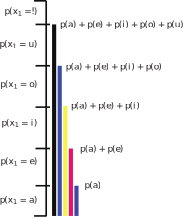
\includegraphics[width=0.3\textwidth]{images/ac_probx.pdf}}
	{Codificação aritmética - exemplo \citep{bilmes2013}.}{fig:ac_probx}
	%\begin{figure}[h!]
	%\centering
	%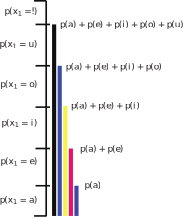
\includegraphics[width=0.3\textwidth]{images/ac_probx.pdf}
	%\label{fig:ac_probx}
	%\end{figure}
  \item Cada subintervalo pode ser subdividido em segmentos de comprimento relativo $p(X_2 = x_2 | X_1 = x_1)$ ou
	comprimento efetivo $p(X_2 = x_2, X_1 = x_1)$.
  \item Os comprimentos relativos podem ser maiores, menores ou iguais, ou seja, $p(X_2 = x_2) \gtreqless p(X_2 = x_2 | X_1 = x_1)$.
  \item A Figura abaixo ilustra as probabilidades considerando que a seguinte sequência ocorreu $x_1 = a, x_2 = e, x_3 = i$ \citep{bilmes2013}.
        \begin{figure}[h!]
        \centering
        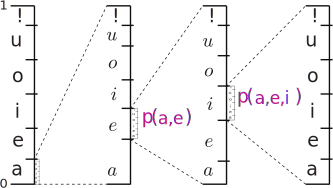
\includegraphics[width=0.65\textwidth]{images/probxacoding.pdf}
        \label{fig:probxacoding}
        \end{figure}
  \item O comprimento absoluto para a sequência `ae' é $p(X_1 = a, X_2 = e) = p(X_1 = a) p(X_2 = e \mid X_1 = a)$.
  \item Os intervalos tornam-se exponencialmente menores com $n$.
  \item A cada passo, os comprimentos relativos podem mudar dependendo do passado.
	No instante $t=1$, o comprimento relativo para `a' era $p(a)$;
	em $t=2$, o comprimento relativo para `a' será $p(a \mid X_1)$, que pode
	mudar dependendo do valor que $X_1$ assumiu.
  \item O número de bits necessários para especificar um determinado sub-intervalo é
	aproximadamente o mesmo que anteriormente, ou seja, o número de bits que serão
	acrescentados em cada etapa é aproximadamente o mesmo. 
	Será o mesmo se os comprimentos relativos não mudarem, ou seja, se 
	a probabilidade condicional não mudar.
  \item Se um símbolo fica muito provável, o comprimento relativo do intervalo é grande
	e assim utilizará poucos bits; por outro lado, se um símbolo torna-se pouco provável,
	o comprimento relativo do intervalo diminui e serão necessários mais bits para 
	distinguir este símbolo. (Exemplo: o intervalo correspondente a $[0.0110,0.0111)$ é 
	menor do que o intervalo correspondente a $[0.10,0.11)$.)
  \end{itemize}

  \framebreak

  \begin{itemize}
  \item Procedimento para codificar.
  \item Para o $i$-ésimo símbolo $X_i$, considere
	\begin{itemize}
	\item o limite inferior do intervalo
		\begin{equation}
		L_n(i \mid x_1, x_2, \ldots, x_{n-1}) = \sum_{j=1}^{i-1} p(x_n = j \mid x_1, x_2, \ldots, x_{n-1})
		\end{equation} 
	\item o limite superior do intervalo
		\begin{equation}
		U_n(i \mid x_1, x_2, \ldots, x_{n-1}) = \sum_{j=1}^{i} p(x_n = j \mid x_1, x_2, \ldots, x_{n-1})
		\end{equation}
	\item Note que $U_n = L_n + p(x_n = i \mid x_1, x_2, \ldots, x_{n-1})$, ou seja, teremos $L_n \leq U_n$ com
		igualdade sse $p(x_n = i \mid x_1, x_2, \ldots, x_{n-1}) = 0$.
	\end{itemize}
  \item Para codificar o $n$-ésimo símbolo, iremos dividir o $(n-1)$-ésimo intervalo definido 
	pelo intervalo semiaberto $[L_n, U_n)$.
  \end{itemize}

  \framebreak

  Para o exemplo dado, considere o intervalo inicial $[0,1)$. Este será dividido de acordo com
  as probabilidades dos símbolos.
  \begin{eqnarray}
  a &\leftrightarrow& [L_1(a), U_1(a)) = [0, p(X_1=a)) \\
  e &\leftrightarrow& [L_1(e), U_1(e)) = [p(X_1=a), p(X_1=a)+p(X_1=e)) \\
  i &\leftrightarrow& [L_1(i), U_1(i)) = [p(a)+p(e), p(a)+p(e)+p(i)) \\
  o &\leftrightarrow& [L_1(o), U_1(o)) = [p(a)+p(e)+p(i), p(a)+p(e)+p(i)+p(o)) \\
  u &\leftrightarrow& [L_1(u), U_1(u)) = [\sum_{x\in \{a,e,i,o\}} p(x), \sum_{x\in \{a,e,i,o,u\}} p(x) ) \\
  ! &\leftrightarrow& [L_1(!), U_1(!)) = [\sum_{x\in \{a,e,i,o,u\}} p(x), 1)
  \end{eqnarray}

  \framebreak

  \begin{itemize}
  \item Vamos utilizar o algoritmo abaixo para codificar uma \textit{string} $x_1, x_2, \ldots, x_N$.
  \item Para tanto iremos determinar os intervalos $[l,u)$ em cada passo $t$, onde $l$ é o limite
	inferior e $u$ o limite superior.
  \end{itemize}

  \begin{algorithmic}
  \State $l\gets 0$
  \State $u\gets 1$
  \State $p\gets u-l$ \Comment{neste caso será 1}
  \For{n = 1 ... N} 
	\Comment{calcule $\forall i \in \mathcal{X}$, $U_n$ e $L_n$ como dado acima}
	\State $u\gets l + p U_n(x_n \mid x_1, \ldots, x_{n-1})$
	\State $l\gets l + p L_n(x_n \mid x_1, \ldots, x_{n-1})$
	\State $p\gets u - l$
  \EndFor 
  \end{algorithmic}

  \begin{itemize}
  \item Ao final de $N$ iterações, teremos um intervalo final $[l,u)$. 
 	Para codificar, basta transmitir uma \textit{string} binária qualquer de um número neste intervalo.
  \item Por outro lado, é possível gerar a sequência binária em tempo de execução, para tanto iremos
	começar a escrever os bits à medida que sabemos, de forma não ambígua, que estamos em um determinado intervalo.
  \item De forma análoga à codificação de Shannon-Fano-Elias, se o intervalo atual é $[0.100101, 0.100110)$, podemos
	enviar os bits que constituem o prefixo comum $1001$, já que isto não será alterado, independente do que ocorrer depois.
  \end{itemize}

  \framebreak

  \begin{example}[\citep{mackay2003}]
  Suponha $x \in \{a,b,\square\}$, onde $\square$ é o símbolo de término.
  
  \begin{itemize}
  \item Vamos considerar a codificação da \textit{string} $bbba\square$.
  \begin{tabular}{cccc}
  -  & $p(a) = 0.425$ & $p(b) = 0.425$ & $p(\square) = 0.15$ \\
  $b$  & $p(a|b) = 0.28$ & $p(b|b) = 0.57$ & $p(\square | b) = 0.15$ \\
  $bb$ & $p(a|bb) = 0.21$ & $p(b|bb) = 0.64$ & $p(\square | bb) = 0.15$ \\
  $bbb$ & $p(a|bbb) = 0.17$ & $p(b|bbb) = 0.68$ & $p(\square | bbb) = 0.15$ \\
  $bbba$ & $p(a|bbba) = 0.28$ & $p(b|bbba) = 0.57$ & $p(\square | bbba) = 0.15$ 
  \end{tabular}
  \end{itemize}

  \examplebreak

  \begin{itemize} 
  \item A figura ilustra os intervalos que teremos ao final da sequência $bbba\square$.

        \begin{figure}[h!]
        \centering
        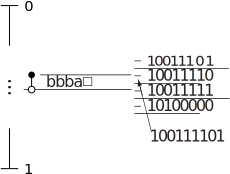
\includegraphics[width=0.3\textwidth]{images/bbba.pdf}
        \label{fig:bbba}
        \end{figure}
  \end{itemize}

  \examplebreak

  \begin{itemize}
  \item Temos subintervalos semiabertos em $[0,1)$.
  \item Os intervalos $[l,u)$ são dados pela probabilidade condicional $p(x_i | x_1, x_2, \ldots, x_{i-1})$. 
  \item Temos a representação de um prefixo $b_1 b_2 \ldots b_k$ por um intervalo da forma
	$[0.b_1 b_2 \ldots b_k, 0.b_1 b_2 \ldots b_k + 2^{-k})$ para $b_i \in \{0,1\}$.
  \item A palavra gerada pela codificação será $100111101$, que determina um intervalo dentro do 
	intervalo final. 
  \end{itemize}

  \examplebreak

	\vspace{-0.5cm}
        \begin{figure}[h!]
        \centering
        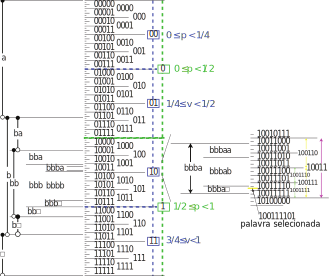
\includegraphics[width=0.5\textwidth]{images/bbbaall.pdf}
        \label{fig:bbbaall}
        \end{figure}

  \end{example}

  \framebreak

  \begin{itemize}
  \item Decodificação.
  \item Para decodificar uma \textit{string} $\alpha=0.z_1 z_2 z_3 \ldots$ utilizaremos o seguinte algoritmo:
  \end{itemize}

  \begin{algorithmic}
  \State $l\gets 0$
  \State $u\gets 1$
  \State $p\gets u-l$ 
  \While{não receber o simbolo final $\square$}
        \State encontre $i$ tal que
	$L_n(i|x_1, \ldots, x_{n-1}) \leq \frac{\alpha - l}{u - l} < U_n(i|x_1, \ldots, x_{n-1}) $ 
        \State $u\gets l + p U_n(i \mid x_1, \ldots, x_{n-1})$
        \State $l\gets l + p L_n(i \mid x_1, \ldots, x_{n-1})$
        \State $p\gets u - l$
  \EndWhile
  \end{algorithmic}

  \framebreak

  \begin{itemize}
  \item Determinação do número de bits.
  \item Um determinado número no intervalo final $[L_n, U_n)$ pode ser arbitrariamente longo. 
	Precisaremos enviar apenas o suficiente para identificar a \textit{string} original de forma univoca. 
  \item Defina
	\begin{equation}
	F_n(i \mid x_1, x_2, \ldots, x_{n-1}) = \frac{1}{2} [L_n(i) + U_n(i)] ,
	\end{equation}
	e $\lfloor F_n(i \mid x_1, x_2, \ldots, x_{n-1}) \rfloor_{l}$ é $F_n$ truncado com $l$ bits.
  \item Poderíamos definir a número de bits utilizado em cada estágio
	\begin{equation}
	l(x_n | x_1, \ldots, x_{n-1}) = \lceil \log 1/p(x_n | x_1, \ldots, x_{n-1}) \rceil + 1 .
	\end{equation}
  \item Ao invés disso, utilizaremos o comprimento de Shannon para o código inteiro
	\begin{equation}
	l(x_{1:n}) = \lceil \log 1/p(x_{1:n}) \rceil + 1 .
        \end{equation}
	À medida que os símbolos chegam ao codificador, é possível calcular
	\begin{equation}
	p(x_{1:n}) = \prod_{i=1}^{n} p(x_i | x_1, \ldots, x_{i-1})
        \end{equation}
	Assim, a cada passo, saberemos quantos bits a mais são necessários em cada passo.
  \item Pelo mesmo argumento dado no código de Shannon-Fano-Elias, teremos um código de prefixo
	e desta forma, unicamente decodificável.
  \item O comprimento esperado será dado por
	\begin{eqnarray}
	E l(x_{1:n}) &=& \sum_{x_{1:n}} p(x_{1:n}) l(x_{1:n}) \nonumber \\
		&=& \sum_{x_{1:n}} p(x_{1:n}) \left( \lceil \log 1/p(x_{1:n}) \rceil + 1 \right) \nonumber \\
		&\leq& - \sum_{x_{1:n}} p(x_{1:n}) ( \log p(x_{1:n}) + 2 ) \nonumber \\
		&=& H(x_{1:n}) + 2
	\end{eqnarray}
  \item Por símbolo teremos $E l \leq H(x_{1:n})/n + 2/n \rightarrow H(\mathcal{X})$.
  \item Temos um \textit{stream code} $\neq$ \textit{block code}.
  \item Ainda temos o problema de estimar $p(x_n | x_1, \ldots, x_{n-1})$.
  \item Outro problema é que os valores das probabilidades ficam exponencialmente pequenos, podendo ocorrer erro de
	precisão numérica. É necessário então expandir os intervalos de tempos em tempos.
  \end{itemize}
\end{frame}


 
\begin{frame}[allowframebreaks]
  \frametitle{Estimar $p(x_n | x_1, \ldots, x_{n-1})$}
  \begin{itemize}
  \item Ainda temos o problema de estimar $p(x_n | x_1, \ldots, x_{n-1})$.
  \item Vamos utilizar um modelo adaptativo.
	\begin{itemize}
	\item Modelo de Dirichlet
		\begin{equation}
		p(a \mid x_{1:n-1}) = \frac{N(a|x_{1:n-1}) + \alpha}{ \sum_{a'} \left( N(a' \mid x_{1:n-1}) + \alpha \right) }
		\end{equation}
		onde $\alpha \geq 0$.
	\end{itemize}
  \item Temos um problema de estimação de densidade.
  \end{itemize}
\end{frame}



\begin{frame}[allowframebreaks]
  \frametitle{Regra de Laplace: derivação Bayesiana}
  \begin{itemize}
  \item Vamos assumir um alfabeto binário $\mathcal{X} = \{0,1\}$.
  \item O número de ocorrências de $0$ e $1$ são dados respectivamente por
	\begin{equation}
	N_0 = N(0|x_{1:n}) \quad \text{ e } \quad N_1 = N(1|x_{1:n}) ,
	\end{equation}	
	sendo que $n=N_0 + N_1$.
  \item Vamos assumir $p_0$, $p_1$ e $p_\square$ as probabilidades para ps símbolos $0$, $1$ e o símbolo terminal $\square$.
  \item O comprimento de uma \textit{string} possui distribuição geométrica
	\begin{equation}
	p(l) = (1 - p_\square)^l p_\square .
	\end{equation}
	Desta forma, $\E l = 1/p_\square$ e $\Var(l) = (1 - p_\square)/p^2_\square$.
  \item As realizações das v.a.s na sequência $X_{1:N}$ são i.i.d.,  desta forma teremos
	\begin{equation}
	p(x_{1:N} \mid p_0, N) = p_0^{N_0} p_1^{N_1} .
	\end{equation}
	Esta é a função de verossimilhança dos parâmetros dados os dados.
  \item Vamos utilizar que \emph{a priori} temos distribuição uniforme, i.e., $\Pr(p_0) = 1$ para $p_0 \in [0,1]$.
	Note que isto é feito para descrever a incerteza com relação à real distribuição que nos é desconhecida.
	A distribuição $p$ não é aleatória, mas incerta. Atribuímos uma distribuição a $p$ para expressar a
	incerteza, não para atribuir aleatoriedade a $p$; mas, matematicamente, será tratado da mesma forma,
	como se a distribuição $p$ fosse aleatória. 
  \item Teremos assim
	\begin{eqnarray}
	\Pr(p_0 \mid x_{1:n}, N) &=& \frac{ \Pr(x_{1:n} \mid p_0, N) \Pr(p_0) }{ \Pr (x_{1:n} \mid N) } \nonumber \\
		&=& \frac{ p_0^{N_0} p_1^{N_1} }{ \Pr (x_{1:n} \mid N) }
	\end{eqnarray}
  \item Vamos utilizar a integral Beta dada a seguir
	\begin{equation}
	B(a,b) \equiv \int x^{a-1} (1-x)^{b-1} dx = \frac{ \Gamma(a) \Gamma(b)}{ \Gamma(a+b)} ,
        \end{equation}
	onde $\Gamma(\cdot)$ é a função gamma, uma extensão da função fatorial, com argumento deslocado de 1.
	Para $n$ inteiro, teremos $\Gamma(n) = (n-1)!$. A função gamma é definida para todos números complexos,
	exceto os inteiros não positivos, pela seguinte integral impropria convergente:
	\begin{equation}
	\Gamma(t) = \int_0^\infty x^{t-1} e^{-x} dx .
	\end{equation}
  \item Utilizando a função Beta, teremos
	\begin{eqnarray}
	\Pr (x_{1:n} \mid N) &=& \int_0^1 \Pr (x_{1:n}, p_0 \mid N) dp_0 = \int_0^1 p_0^{N_0} p_1^{N_1} \Pr(p_0) dp_0 \nonumber \\
		&=& \frac{\Gamma(N_0 + 1) \Gamma(N_1 + 1)}{ \Gamma(N_0 + N_1 + 2) } = \frac{ N_0! N_1! }{ (N_0 + N_1 +1)! }
        \end{eqnarray}
  \item Para realizar a predição, queremos saber qual é a probabilidade do próximo símbolo ser igual a $0$, por exemplo, 
	dado que temos uma sequência de $N$ observações, ou seja,
	\begin{eqnarray}
	\Pr(X_{n+1} = 0 \mid x_{1:n},N) &=& \int_0^1 \underbrace{ \Pr(0 \mid p_0) }_{ = p_0} \Pr(p_0 \mid x_{1:n}, N) dp_0 \nonumber \\
			&=& \int_0^1 p_0 \frac{p_0^{N_0} p_1^{N_1}}{\Pr(x_{1:n} \mid N)} dp_0 \nonumber \\
			&=& \int_0^1 \frac{p_0^{N_0 +1} p_1^{N_1}}{\Pr(x_{1:n} \mid N)} dp_0 \nonumber \\
			&=& \left( \frac{(N_0 + 1)! N_1!}{(N_0 + N_1 + 2)!} \right) / \left( \frac{ N_0! N_1! }{ (N_0 + N_1 +1)!  } \right) \nonumber \\
			&=& \frac{ N_0 + 1  }{ N_0 + N_1 + 2}  \quad \text{regra de Laplace}
        \end{eqnarray}
  \end{itemize}

  \framebreak

  \begin{itemize}
  \item Para a abordagem de Dirichlet, teremos a seguinte aproximação:
	\begin{equation}
	Pr(X_{n+1} = 0 \mid x_{1:n},N) = \frac{ N_0 + \alpha  }{ N_0 + N_1 + 2\alpha}
	\end{equation} 

  \item Para calcular esta probabilidade ao longo do processo de codificação, não será necessário armazenar toda
	a história, mas apenas alguma estatística sobre os dados, como por exemplo, o número de ocorrências de cada símbolo.
  \end{itemize}

  \framebreak

  \begin{block}{Regra da Sucessão}
  Regra da Sucessão é a formulação introduzida no Século XVIII por Pierre-Simon Laplace para lidar com o `problema do nascer do sol'. 

  Se repetirmos um experimento, que sabemos previamente que pode resultar em sucesso ou falha, $n$ vezes de forma independente e 
  observamos $s$ sucessos, então como podemos estimar a probabilidade de que a próxima realização será um sucesso? 
  (Qual é a probabilidade de que o sol nascerá amanhã, visto que nos últimos 5 mil anos, ou 1826251 dias, foi observado que o sol nasceu todas as vezes?) 
  \blockbreak
  Ou seja, se $X_1, \ldots, X_{n+1}$ são v.a.s condicionalmente independentes, que assumem valor $0$ ou $1$, então, se não sabemos nada além disso,
  teremos
	\begin{equation}
	P(X_{n+1} = 1 \mid X_1 + \ldots + X_n = s) = \frac{ s+ 1}{n+2} .
	\end{equation}
  Note que, se não soubéssemos que ambos, sucesso e fracasso, são possíveis, então teríamos a seguinte probabilidade
        \begin{equation}
        P'(X_{n+1} = 1 \mid X_1 + \ldots + X_n = s) = \frac{s}{n} .
        \end{equation}
  \blockbreak
  Seja $X_i = 1$ se observamos um sucesso na $i$-ésima realização da v.a. e $0$ caso contrário, com probabilidade $p$ de sucesso,
  teremos então uma distribuição de Bernoulli. Vamos supor que $X_1 , \ldots, X_n$ são independentes, dado $p$.
  Pelo teorema de Bayes, para encontrar a distribuição de probabilidade condicional de $p$ dado $X_i$, $i=1,\ldots,n$, devemos
  multiplicar a medida da probabilidade a priori dada a $p$ pela função de verosimilhança 
	\begin{equation}
	L(p) = P(X_1 = x_1, \ldots, X_n = x_n \mid p) = \prod_{i=1}^n p^{x_i} (1-p)^{1-x_i} = p^s (1-p)^{n-s}
        \end{equation}
  onde $s=x_1 + \ldots + x_n$ é o número de sucessos e $n$ o número de tentativas.
  \blockbreak
  A função densidade de probabilidade a priori que expressa ignorância total sobre $p$ (exceto pela fato de que sabemos
  que não é $1$, nem $0$, ou seja, existem duas possibilidades de fato: sucesso ou falha) é uniforme, sendo igual a
  $1$ para $0 < p < 1$ e $0$ (zero) caso contrário. Para obter a constante de normalização faremos
        \begin{equation}
	\int_0^1 p^s(1-p)^{n-s} dp = \frac{s! (n-s)!}{(n+1)!}
        \end{equation}
  \blockbreak
  A função densidade de probabilidade a posteriori é dada pelo produto da função densidade de probabilidade a priori com a 
  função de verossimilhança e normalizando. Teremos assim
        \begin{equation}
	f(p) = \frac{(n+1)!}{s! (n-s)!} p^s (1-p)^{n-s} .
        \end{equation}
  Esta é a distribuição beta com valor esperado
        \begin{equation}
	\int_0^1 p f(p) dp = \frac{s+1}{n+2} .
        \end{equation} 
  \blockbreak
  Como a probabilidade condicional de sucesso na próxima realização, dado o valor de $p$, é apenas $p$, a lei da probabilidade total
  diz que a probabilidade de sucesso na próxima realização é apenas o valor esperado de $p$. Como tudo isto é condicional aos dados
  observados $X_i$, para $i=1,\ldots,n$, temos
        \begin{equation}
	P(X_{n+1} = 1 \mid X_1 = x_1, \ldots, X_n = x_n ) = \frac{s + 1}{n + 2} .
        \end{equation}
  \end{block}

\end{frame}
